\section{Question 4.2}

\subsection{Question}
Plot vocabulary growth for the Wikipedia collection and estimate the parameters for Heaps' law. Should the order in which the documents are processed make any difference?

\subsection{Approach}
The \texttt{filevisitor.py} script, found in Listing \ref{listing:filevisitor}, was modified to also log the vocabulary and total word count after visiting each document in the small Wikipedia collection.  The graphvocab.R script found in Listing \ref{listing:graphvocab} was then used to create the Vocabulary Growth graph, which can be found in Figure \ref{fig:vocab}.

\begin{figure}[h!]
\centering
\label{fig:vocab}
\fbox{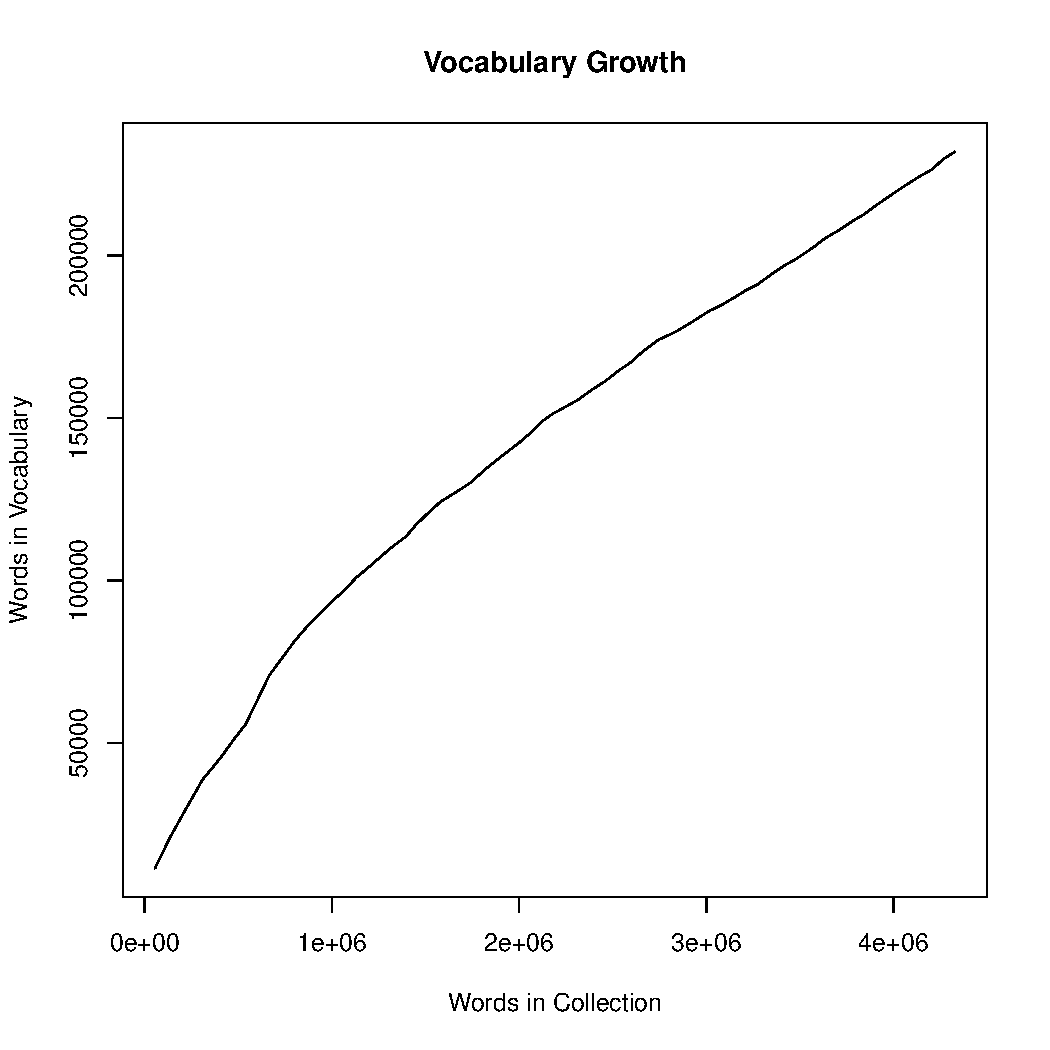
\includegraphics[scale=.55]{code/Rscripts/vocab.pdf}}
\caption{Vocabulary Growth for the Small Wikipedia Collection}
\end{figure}